\documentclass[10pt, aspectratio=169]{beamer}
\usepackage{kinetic}
\usetikzlibrary{arrows.meta}
\setbeamertemplate{navigation symbols}{}

\colorlet{tierA}{blue}
\colorlet{tierB}{green!60!black}
\colorlet{tierC}{red!80!black}

\tikzset{
  >={Stealth[round]},
  diagram/.style={font=\scriptsize, every node/.style={align=center}},
  outerbox/.style={rounded corners=2pt, line width=0.9pt},
  block/.style={rounded corners=1.5pt, line width=0.8pt},
  title/.style={anchor=north west, font=\footnotesize\bfseries},
  bigtitle/.style={anchor=north west, font=\Large\bfseries},
  badge/.style={anchor=north east, font=\scriptsize\itshape, text=black!65},
  iface/.style={->, line width=1.2pt},
  ifacelabel/.style={font=\scriptsize, fill=white, inner sep=1.5pt},
  sub/.style={block, font=\footnotesize, text=black},
}
\newcommand{\canvas}{\useasboundingbox (-1.3,-0.2) rectangle (12.4,4.7);}

% #1: overlay specification for the arrows
\newcommand{\overview}[1]{%
  \fill[outerbox, tierA!8, draw=tierA] (0,2.55) rectangle (5,4.55);
  \node[title, text=tierA!60!black] at (0.12,4.54) {Source};
  \node[badge] at (4.88,4.54) {\texttt{.tex}};
  \fill[outerbox, tierA!18, draw=tierA] (0.35,2.65) rectangle (4.65,4.12);
  \node[title] at (0.47,4.10) {Beamer deck};
  \draw[block, fill=tierA!32, draw=tierA] (0.7,2.73) rectangle (4.3,3.65);
  \node at (2.5,3.19) {\textbf{TikZ scopes}\\ named with\\ morph, move, zoom};
  \begin{scope}[zoom=build]
    \fill[outerbox, tierB!10, draw=tierB] (7.6,2.55) rectangle (12.1,4.55);
  \end{scope}
  \node[title, text=tierB!55!black] at (7.72,4.47) {Build};
  \node[badge] at (11.98,4.47) {\texttt{kinetic}};
  \draw[block, fill=tierB!28, draw=tierB] (8.1,2.85) rectangle (11.6,3.95);
  \node at (9.85,3.4) {\textbf{dvisvgm}\\ one SVG per page};
  \fill[outerbox, tierC!10, draw=tierC] (0,0.08) rectangle (12.1,1.7);
  \node[title, text=tierC!60!black] at (0.12,1.62) {Outputs};
  \node[badge] at (11.98,1.62) {two files};
  \draw[block, fill=tierC!24, draw=tierC] (0.6,0.18) rectangle (5.7,1.1);
  \node at (3.15,0.64) {\textbf{PDF}\\ static overlays};
  \begin{scope}[morph=deck]
    \draw[block, fill=tierC!24, draw=tierC] (6.4,0.18) rectangle (11.5,1.1);
  \end{scope}
  \begin{scope}[move=decktitle]
    \node[font=\scriptsize\bfseries] at (8.95,0.88) {HTML deck};
  \end{scope}
  \node[inner sep=0pt] at (8.95,0.5) {animated};
  \only<#1>{%
    \begin{scope}[drawon=dvi]
      \draw[iface, tierA!60!black] (4.65,3.4) -- (7.6,3.4);
      \node[ifacelabel] at (6.125,3.4) {\textbf{latex}:\\ DVI with\\ named groups};
    \end{scope}
    \begin{scope}[drawon=html]
      \draw[iface, tierB!55!black] (9.85,2.55) -- (9.85,1.7);
      \node[ifacelabel] at (9.85,2.125) {\textbf{one HTML file}};
    \end{scope}
    \begin{scope}[drawon=pdf]
      \draw[iface, tierA!60!black] (0,3.5) -- (-0.9,3.5) -- (-0.9,0.6) -- (0,0.6);
      \node[ifacelabel, rotate=90] at (-0.9,2.05) {\textbf{pdflatex}: PDF};
    \end{scope}}%
}

\title{kinetic showcase}
\subtitle{Animated Beamer slides in the browser}
\date{}

\begin{document}

\begin{frame}
  \titlepage
\end{frame}

\begin{frame}{From One Source to Two Outputs}
  \centering
  \begin{tikzpicture}[diagram]\canvas\overview{2-}\end{tikzpicture}

  \vspace{1em}
  \only<1>{One source file, one build command, two outputs.}%
  \only<2>{Draw-on: the arrows appear stroke by stroke.}
\end{frame}

\begin{frame}{Inside the HTML Deck}
  \centering
  \begin{tikzpicture}[diagram]\canvas
    \begin{scope}[morph=deck]
      \draw[block, fill=tierC!10, draw=tierC] (-1.2,-0.1) rectangle (12.3,4.6);
    \end{scope}
    \begin{scope}[move=decktitle]
      \node[bigtitle, text=tierC!60!black] at (-1.0,4.5) {HTML deck};
    \end{scope}
    \begin{scope}[fade=parts]
      \draw[sub, fill=tierC!24, draw=tierC] (-0.6,1.2) rectangle (2.4,2.6);
      \node[font=\footnotesize] at (0.9,1.9) {\textbf{Pages}\\ inline SVG};
      \draw[sub, fill=tierC!24, draw=tierC] (3.4,0.6) rectangle (8.2,3.2);
      \node[font=\footnotesize] at (5.8,2.85) {\textbf{Viewer}};
      \draw[sub, fill=tierC!24, draw=tierC] (9.2,1.2) rectangle (12.0,2.6);
      \node[font=\footnotesize] at (10.6,1.9) {\textbf{Screen}\\ full screen};
    \end{scope}
    \only<3->{%
      \begin{scope}[fade=kinds]
        \draw[sub, fill=orange!35, draw=orange] (3.7,0.8) rectangle (5.7,2.4);
        \node[font=\scriptsize] at (4.7,1.6) {morph\\ and move};
        \draw[sub, fill=green!30, draw=green!60!black] (5.9,0.8) rectangle (7.9,2.4);
        \node[font=\scriptsize] at (6.9,1.6) {zoom\\ and fade};
      \end{scope}}
    \only<2->{%
      \begin{scope}[drawon=flow]
        \draw[iface, black!60] (2.4,1.9) -- (3.4,1.9);
        \draw[iface, black!60] (8.2,1.9) -- (9.2,1.9);
      \end{scope}}
    \only<4->{%
      \begin{scope}[drawon=inputs]
        \draw[iface, tierA!60!black] (4.7,4.4) -- (4.7,3.2);
        \node[ifacelabel] at (4.7,3.85) {\textbf{names}};
        \draw[iface, tierB!55!black] (6.9,4.4) -- (6.9,3.2);
        \node[ifacelabel] at (6.9,3.85) {\textbf{keys}};
      \end{scope}}
  \end{tikzpicture}

  \vspace{1em}
  \only<1>{Staged morph: the rest fades out, the block grows, the detail fades in.}%
  \only<2>{Fade and draw-on: the parts appear.}%
  \only<3>{The viewer runs one kind of animation per page change.}%
  \only<4>{The names come from the TikZ keys. The arrow keys drive the deck.}
\end{frame}

\begin{frame}{From One Source to Two Outputs}
  \centering
  \begin{tikzpicture}[diagram]\canvas\overview{1-}\end{tikzpicture}

  \vspace{1em}
  Next: a camera zoom into the build, for comparison.
\end{frame}

\begin{frame}{Inside the Build}
  \centering
  \begin{tikzpicture}[diagram]\canvas
    \begin{scope}[zoom=build]
      \fill[outerbox, tierB!10, draw=tierB] (-1.2,-0.1) rectangle (12.3,4.6);
    \end{scope}
    \node[bigtitle, text=tierB!55!black] at (-1.0,4.5) {Build};
    \draw[sub, fill=tierB!20, draw=tierB] (-0.6,0.2) rectangle (11.7,1.0);
    \node[font=\footnotesize] at (5.55,0.6) {\textbf{latex}: DVI with named groups};
    \draw[sub, fill=tierB!20, draw=tierB] (-0.6,1.4) rectangle (2.8,3.4);
    \node[font=\footnotesize] at (1.1,2.4) {\textbf{dvisvgm}\\ SVG pages};
    \draw[sub, fill=tierB!20, draw=tierB] (8.3,1.4) rectangle (11.7,3.4);
    \node[font=\footnotesize] at (10.0,2.4) {\textbf{Images}\\ embedded};
    \only<2->{%
      \begin{scope}[fade=assembly]
        \draw[sub, fill=tierB!40, draw=tierB] (3.4,1.4) rectangle (7.7,3.4);
        \node[font=\footnotesize] at (5.55,2.4) {\textbf{HTML assembly}\\ pages, images,\\ viewer};
      \end{scope}}
    \only<3->{%
      \begin{scope}[drawon=buildflow]
        \draw[iface, <->, black!60] (5.55,1.0) -- (5.55,1.4);
        \draw[iface, <->, black!60] (2.8,2.4) -- (3.4,2.4);
        \draw[iface, <->, black!60] (7.7,2.4) -- (8.3,2.4);
      \end{scope}}
  \end{tikzpicture}

  \vspace{1em}
  \only<1>{Camera zoom: the view moves into the block, then the detail fades in.}%
  \only<2>{The build puts pages, images, and the viewer into one file.}%
  \only<3>{Press the left arrow to zoom back out.}
\end{frame}

\begin{frame}{Default Animation Durations}
  \kntransition{push}
  \centering
  \begin{tikzpicture}[font=\footnotesize]
    \useasboundingbox (-1,-0.8) rectangle (11,5);
    \draw[black!50] (0,0) -- (10,0);
    \foreach \x/\h/\c/\n in {1/2.33/tierA/a, 3.5/4.33/tierA/b, 6/3.33/tierB/c, 8.5/1.83/tierC/d}{
      \begin{scope}[morph=bar\n]
        \only<1>{\fill[\c] (\x-0.6,0) rectangle (\x+0.6,0.05);}
        \only<2->{\fill[\c] (\x-0.6,0) rectangle (\x+0.6,\h);}
      \end{scope}}
    \node at (1,-0.45) {morph};
    \node at (3.5,-0.45) {staged morph};
    \node at (6,-0.45) {camera zoom};
    \node at (8.5,-0.45) {push};
    \only<2->{\foreach \x/\h/\v in {1/2.33/700, 3.5/4.33/1300, 6/3.33/1000, 8.5/1.83/550}{
      \node[above] at (\x,\h) {\v\,ms};}}
  \end{tikzpicture}

  \only<1>{Push transition into this frame.}%
  \only<2>{Grow: each bar morphs from a flat copy.}
\end{frame}

\begin{frame}{PDF Figures}
  \centering
  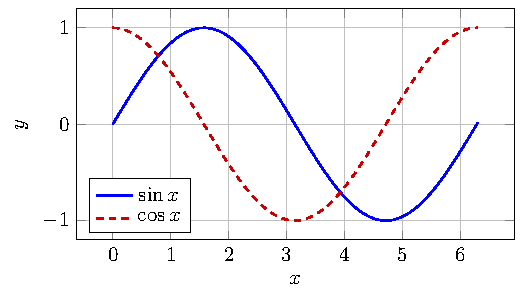
\includegraphics[width=0.7\textwidth]{figures/plot}

  This plot is a PDF file. The HTML build converts it to SVG with \texttt{pdftocairo}.
\end{frame}

\begin{frame}[fragile]{How the Morph Is Written}
  \kntransition{fade}
  Give a scope the same name on two consecutive pages:
\begin{semiverbatim}\small
\\only<1>\{\\begin\{scope\}[morph=box]
  \\fill[blue] (0,0) circle (1);\\end\{scope\}\}
\\only<2>\{\\begin\{scope\}[morph=box]
  \\fill[red] (2,0) rectangle (5,2);\\end\{scope\}\}
\end{semiverbatim}
  The PDF shows the two overlays. The HTML deck morphs the circle into the rectangle.
\end{frame}

\begin{frame}{Harder Morph Cases}
  \centering
  \begin{tikzpicture}[font=\footnotesize]
    \useasboundingbox (-1.5,-1.6) rectangle (12.5,1.8);
    \begin{scope}[morph=ring]
      \only<1>{\fill[tierA, even odd rule] (0,0) circle (1) (0,0) circle (0.5);}
      \only<2>{\fill[tierA, even odd rule] (1,0) circle (0.8) (1,0) circle (0.4);}
    \end{scope}
    \begin{scope}[morph=curve]
      \only<1>{\draw[tierB, line width=1.5pt] (3.5,0) .. controls (4.5,1.5) and (5.5,-1.5) .. (6.5,0);}
      \only<2>{\draw[tierB, line width=1.5pt] (3.5,0.5) .. controls (4.5,-1.5) and (5.5,1.5) .. (6.5,0.5);}
    \end{scope}
    \begin{scope}[morph=labeled]
      \only<1>{\draw[tierC, line width=1pt] (8.5,-0.6) rectangle (10.5,0.6);}
      \only<2>{\draw[tierC, line width=1pt] (8.5,-0.6) rectangle (12,0.6);}
      \node at (9.5,0) {label};
    \end{scope}
    \node at (0.5,-1.4) {ring};
    \node at (5,-1.4) {open curve};
    \node at (10.25,-1.4) {label in a morph};
  \end{tikzpicture}

  \vspace{0.5em}
  \begin{itemize}\footnotesize
    \item Ring: each outline morphs on its own, so the hole stays open.
    \item Open curve: the curve stays open and keeps its two end points.
    \item Label: content in a morph scope that does not change stays on screen.
  \end{itemize}
  \only<1>{Press the right arrow to see the three morphs.}%
  \only<2>{Press the left arrow to see the morph in reverse.}
\end{frame}

\begin{frame}{One Source, Two Outputs}
  \kntransition{fade}
  \centering\vfill
  {\Large A PDF for print and for Overleaf,\\[0.3em]
    an HTML deck with motion for the talk.}
  \vfill
  Fade transition into this frame.
\end{frame}

\end{document}
